WWW は情報の公開を目的とした TCP/IP 上のサービスである.近年は,単なる情
報公開にとどまらず,情報検索,電子メール,チャット,地図やルート,時刻表
の検索,ショッピングやオークション,ホテルやチケットの予約など,さまざま
なサービスの基盤としても使用されている.そのため,今日ではインターネット
上のサービスのインフラの一つとなっている.WWW を介して提供されるサービ
スには繊細な情報を扱うものがあり,正当性を確認するための認証技術や第三者
に内容が分からないように情報を変換する暗号化技術が併用される機会も増えて
いる.暗号化技術は認証技術の基盤としても用いられ,WWW 上のセキュリティ確
保のための重要な役割を果たしている.

\section{WWW システム}
World Wide Web (WWW, W3, the Web) は,インターネットにおいて利用されてい
るサービスの一つである.

WWW はインターネット上で情報を公開・流通・閲覧する方法の一つであり,その
根幹をなす概念にハイパーテキスト (hypertext) がある.ハイパーテキストは,
文書を表現するテキストの中の語句に対して,関連する他の文書へ関連付けを定
義し,ユーザはその関連をたどることで,関連する情報を閲覧することができる.
この文書間の関連付けをハイパーリンク (hyperlink) と呼ぶ.現在の WWW では,
テキストのみならず,画像,音声,映像など,多くのコンテンツを表現すること
ができる.また,静的な情報だけでなく,動的な情報,インタラクティブなコン
テンツの流通基盤としても用いられている.

現在の WWW は,1990年,CERN\footnote{the European Organization for
Nuclear Research: 欧州合同素粒子原子核研究機構}の Tim Berners-Lee により
開発され,CERN の研究所内の論文・データ閲覧の手段として用いられた.この
時,Web サーバ (web server, WWW サーバ, HTTP サーバ)および Web ブラウザ
(web browser, Web クライアント, HTTP クライアント) として用いら
れたコンピュータは NeXT コンピュータであった.1993年,
NCSA\footnote{National Center for Supercomputing Applications,
University of Illinois at Urbana-Champaign, イリノイ大学付属 米国立スー
パーコンピュータ応用研究所} の Marc Andreessen\footnote{その後,Netscape 
社を創業} により Web サーバであるNCSA http サーバ,Web ブラウザである 
Mosaic が開発された.1994年には,Tim Berners-Lee により World Wide Web
Consortium (W3C)が設立され,WWW の仕様の標準化などを行うようになった.

現在では,多くの Web ページが公開されており,Web サーバ,Web ブラウザと
も多くのプログラムが提供されるようになっている.

Web サービスを用いた情報公開により,情報公開者はインターネットに情報を公
開することが可能となり,全世界へ広く情報を発信することができる.インター
ネットの利用者は,それら世界中で発信された情報を自由に閲覧することができ
る.

一方で,インターネットが社会一般に広まったことにより,利用者層や利用者の
考え方も様々なものとなっている.それらの中には,悪意を持つ利用者も存在す
る.こうした現在のインターネットの置かれている状況下では,適切な情報の発
信が重要になる.すなわち,公開しても良い情報なのか,公開すべきではない情
報なのかを,個々の情報発信者が気を付ける必要がある.一度インターネットへ
公開された情報は,インターネット上へ広く拡散することになり,仮に,公開す
べきでない情報を公開してしまった場合,この情報を回収することは困難なもの
となる.

また,全世界へ公開するのではなく,一部の利用者のみに限定した情報を公開を
行いたい場合がある.このような場合には,Web サーバのアクセス制限や認証
の機能を用いることで,一部の利用者のみに情報を公開することが可能となる.

WWWを構成する技術として,データ形式を定義する HTML と,そのデータのやり
とりを行うプロトコルである HTTP がある.

\subsection{HTML}
WWW でよく用いられるデータは,HTML (Hyper Text Markup Language) と呼ばれ
る記述形式で書かれた文書である.HTML は,SGML(Standard Generalized Markup 
Language) の書式を踏襲したマークアップ言語である.

HTML は,ハイパーテキストを記述するためのマークアップ言語であり,ハイパー
リンクを用いて他の情報への関連付けを行う.また,通常のテキストに対して,
タグと呼ばれる記法で文書の構造やハイパーリンクなどの要素に関する意味づけ
を行う.

ハイパーリンクは,他の HTML 文書だけでなく,JPEG などの画像情報や,音声,
動画像,テキストファイル,PDF ファイルなど,コンピュータが取り扱う様々な
形式のファイルに関連づけることができる.このためマルチメディア情報を取り
扱うことにも適している.

\subsection{HTTP}

%WWW サービスを実現するために用いられるプロトコルが,HTTP (Hyper Text
%Transfer Protocol) である.HTTP は RFC 2616 で規定され,現在は 1999年に
%策定されたバージョン 1.1 が用いられる.

WWW サービスを実現するために用いられるプロトコルが,HTTP (Hyper Text
Transfer Protocol) である.
HTTP は,Web サーバと Web ブラウザの間で,HTML やその他の様々なファイル
をやりとりするための転送手順を決めている,アプリケーション層プロトコルで
ある.

HTTP は1999年に策定されたバージョン 1.1 において基本的な機能が整備された.
HTTP/1.1 は RFC 2616 として規定されたが,現在では RFC 7230 から RFC 7235 
として整理された.また,多重化などの拡張が施されたバージョンである HTTP/2 
についても RFC 7540 として策定された.

また,HTTP では HTML 以外にも様々な情報の送受信を行うため,それらの属性
を定め,正しく情報の受信側で認識・閲覧・再生できるよう,電子メールでも用
いられる MIME (Multipurpose Internet Mail Extension) によりファイルの属
性を定義し,送信時に通知している.

\subsection{URI}
WWW 上のリソースを一意に表すものとして用いられるのが URI (Uniform Resource 
Identifier) である.URI はプロトコルに依存せず,インターネット上の任意の
ホストの任意の公開情報を指定することが可能である.クライアントは,Web サ
ーバとのコネクションを確立すると,リクエストとして表示したい WWW ページの
 URI を送信する.これに対し Web サーバは,自分が持つその URI の示す文書を
クライアントに送信する.

\begin{cli}
 <スキーム>://(ログイン情報@)<ホスト名>(:ポート)/<絶対パス>
 (例: http://www.kochi-tech.ac.jp/index.html)
\end{cli}

スキームとは,データ取得のために用いる手段であり,具体的には http やftp,
https などのプロトコルを表し,:// の後に,ホスト名\footnote{インターネッ
トでは FQDN (Fully Qualified Domain Name: DNS システムを用いた命名規則に
よる世界唯一のホスト名) を用いる} が続き,パスを絶対パスで記述する.
\footnote{必ずしもサーバ上のファイルシステムのファイルのパスとは限らず,
情報(resource) が一意に (uniformly) 特定 (identify)できさえすれば,何で
も良い} ポート番号は,\texttt{/etc/services} に指定された通りの番号
\footnote{IANA で規定されている番号.HTTP は 80,FTP は 21,HTTPS は 443 
など} である場合は,省略する.

URL (Uniform Resource Locator) は URI のサブセットであり,明示的にリソー
スが存在する場所を指し示したい場合に用いられる.WWW においては,URI とし
て URL が用いられることが多い.

\subsection{HTTP におけるリクエストとレスポンス}

図\ref{fig:04:http}に示すように,HTTP のメッセージは,Web クライアントか
ら Web サーバへの Request と,Web サーバからの返信である Response のやり
とりでデータが交換される.トランスポート層プロトコルとして TCP を用いて
おり,Web サーバのポート番号は 80 が一般に用いられる.

\begin{figure}[ht]
 \begin{center}
  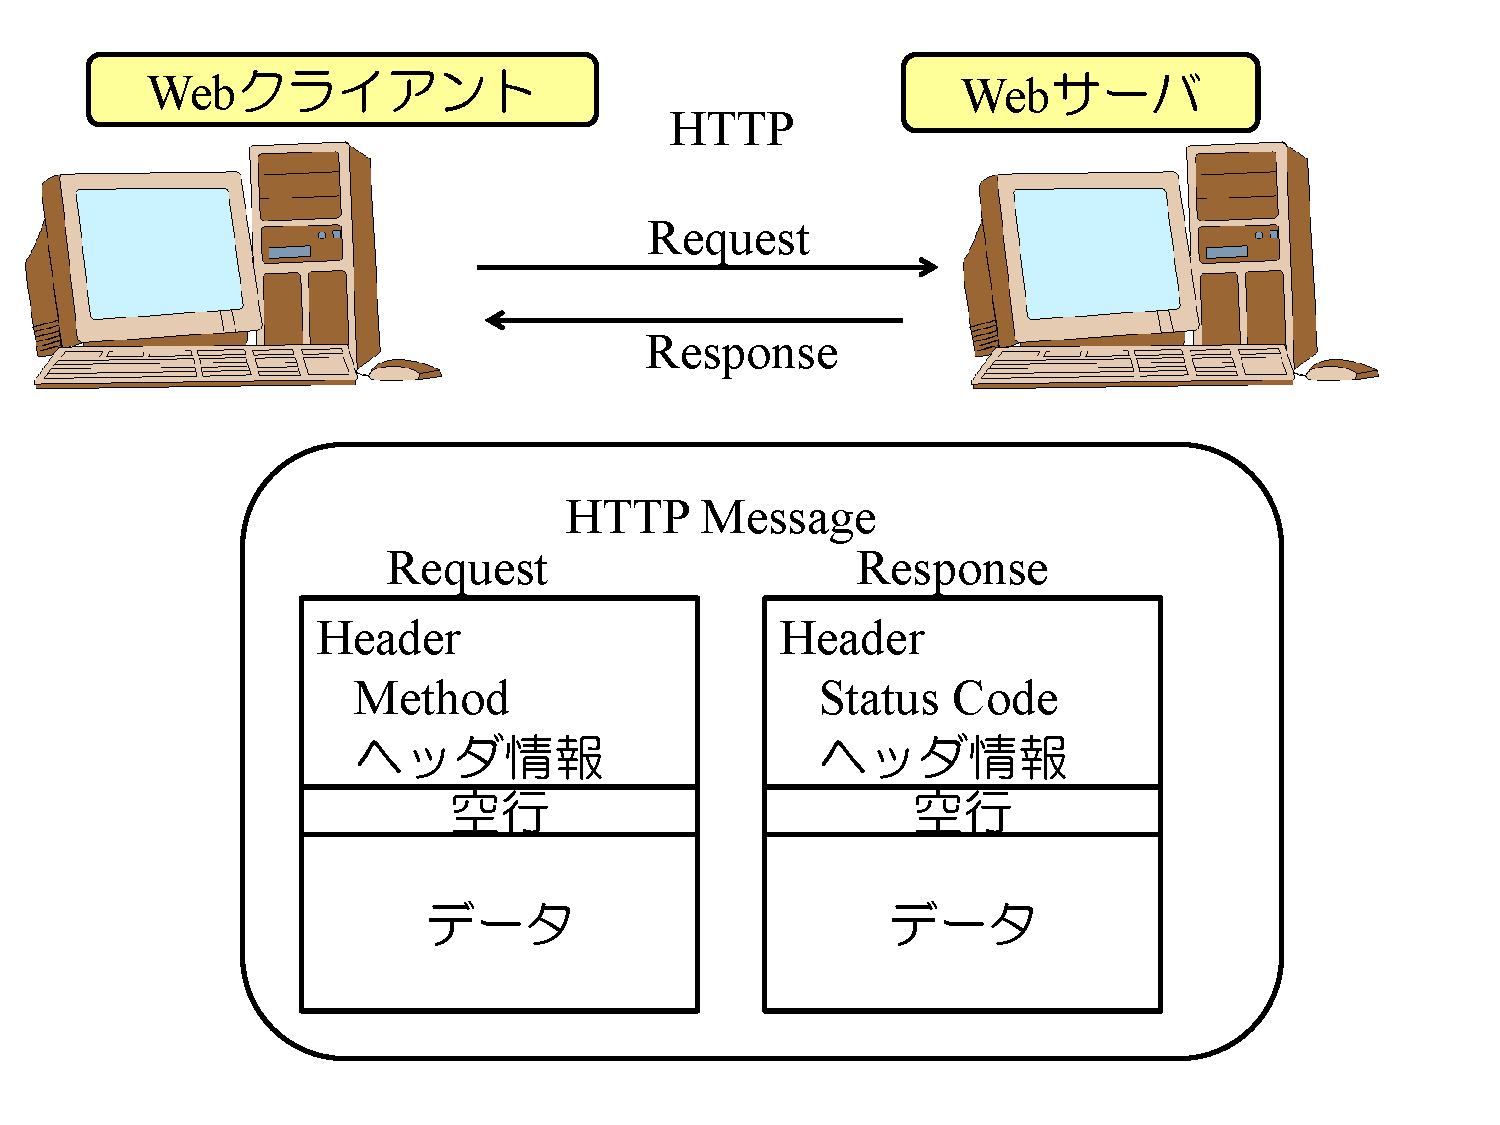
\includegraphics[width=10cm, bb=0 0 720 550, clip]{04_http_auth_crypt/http.pdf}
  \caption{HTTP のプロトコル概要}
  \label{fig:04:http}
 \end{center}
\end{figure}

まず,Web ブラウザは,HTTP Request を Web サーバへ送信する.
HTTP Request は,ヘッダに続き,空行を1行送信した後,送信データがあればデータを送る.
HTTP Request の冒頭にはメソッドと呼ばれるどのような情報交換をのぞむかの指定が含ま
れる.よく用いられるものは,GET(サーバからのデータ取得要求)などである.
それぞれのメソッドでは,データの場所を指定する URI を記述する.
たとえば,Web ブラウザは入力された URL を
\begin{cli}
GET <絶対パス> <メソッド> Host:<ホスト>
(例 GET /index.html HTTP/1.1 Host www.kochi-tech.ac.jp)
\end{cli}
という GET メソッド(ここでは GET だが,他には PUT や POST 等がある)に変換し,
Web サーバへリクエストを送る.

この GET メソッド以外のメソッドには以下のようなものがある.
\begin{description}
 \item[\texttt{HEAD}] \ \\
       識別したURLからHTTPヘッダ情報を検索(取得)する.
 \item[\texttt{POST}] \ \\
       指定したURLにデータを送る.
 \item[\texttt{PUT}]  \ \\
       指定したURLにPOSTされたデータを入れて,既存のデータを置き換える.
\end{description}

HTTP Request を受信したサーバは,HTTP Response を送信する.
HTTP Response もヘッダとデータからなり,空行1行で
隔てられる.ヘッダには,冒頭に Status Code が記述され,Request に対する
結果(状態)を番号で返す.例えば,200 は要求は受理され実行されること,
404 は URI で指定されたデータが存在しないこと,500 はサーバ内でエラーが
生じたことなどを示す.ヘッダには,その他,データの長さ,データの種類(テ
キスト,映像,etc.)や,テキストの文字コード,エンコーディング,データの
タイムスタンプなどが記述され,空行の後,データ本体が続く.

たとえば,Web サーバは,
\begin{cli}
<HEAD>
<TITLE> ..... </TITLE>
:
</BODY>
\end{cli}
というような,HTML のデータを返す
(今述べた「GET /index.html」は,URL として該当する HTML データを要求していることを
表している).
Web ブラウザは受け取った HTML のデータを解析し,表示する.

このような Web サーバとクライアントとの通信の様子は,telnet%
\footnote{ネットワーク経由の仮想端末ソフトウェア} %
を使用して簡単に確認する
ことができる(一般に HTTP のポート番号は 80 番を使用する).


\subsection*{Cookie}
%Content Management System の構築のためには,どのユーザがどのような処理を
%しているかを Web サーバ側で把握するために,\textbf{Cookie} の仕組みが用
%いられる.
HTTP はステートレスなプロトコルであり,
%ブラウザからのリクエストのたびに TCP 接続が行われ,そのリクエストに対するレスポンスが終了する
%と,接続は切断される.次のリクエストに対しては,あらたに TCP 接続が作成される.このため,
サーバからは,個々のリクエストについて同一のユーザか否
かを判定することができない(IP アドレスだけではクライアントを識別する情
報としては不足していることに注意する).Cookie は,このような問題を解決
するために
%HTTP のプロトコルで
定義されている仕組みであり,サーバからブ
ラウザに対して識別情報を送り,ブラウザはその情報を受け入れると,次回の同
一サーバに対する接続から,リクエストにその情報を付与して送る.この情報を
Cookie と呼ぶ.


\subsection{Web サーバの種類}
Web サーバはそもそも学術目的の文献を交換することを目的として
開発された.最初の Web サーバはスイスの欧州粒子物理学研究所(CERN)で
開発された CERN httpd である.

現在,Web サーバのソフトウェアには Microsoft の IIS(Internet Informaiton
Server),Sun Microsystems 社の Java で書かれた Java Web Server,
Igor Sysoev による nginx,そして,Apache などがある.

\subsection*{Apache}

Apache とは NCSA\footnote{National Center Supercomputing} httpd Ver.1.3 を
ベースに,機能拡張が図られた Web サーバである.その特徴は,
機能が豊富で高性能であり,多くのプラットフォームに対応している.

Apache の構成は,モジュールの追加によって行っているので,
必要な機能だけ使用する事ができ,最新の機能もモジュールを追加する事により
簡単に使用することができる.また,メモリ管理がしっかりしており,
速さ・メモリ共に効率的である.Apache は Solaris,Linux などの UNIX はもちろん,
Windows(Win32 版),OS/2 などほとんどの OS で使用することができる.

Apache は HTTP Apache Server Project において開発が行われており
グループのメンバーは,世界中のボランティアで構成されている.
ホームページは \texttt{http://www.apache.org/} である.
%apache の現在の安定したバージョンは 1.3.12 である.
%\setcounter{subsubsection}{0}
%\subsubsection{Apacheの代表的な機能}

Apacheの持つ代表的な機能を以下に示す.

\begin{description}
 \item[Proxy サーバ] \ \\
      Proxy の機能を提供する.

 \item[CGI(Common Gateway Interface)] \ \\
      Web サーバのバックエンドでサーバアプリケーションを動かすとき,
      Web サーバからサーバアプリケーションを呼び出す標準的なインタフェース.

 \item[SSI(Server Side Includes),XSSI(eXtended Server Side Includes)] \ \\
      Web サーバの機能の一つで,HTML ファイル中に別のファイルの内容やプログ
      ラムの実行結果を挿入する機能.
      XSSI は SSI の拡張機能.

 \item[バーチャルホスト] \ \\
      サービスホストが複数の IP アドレスをもったマルチホームホストである場合
      や,複数のドメインホスト名を持っている場合に,リクエストを受けた %
      IP アドレスごと,あるいは HTTP リクエストの Host:フィールドの値ごとに
      異なる設定のサービスを行う機能.

 \item[認証機能] \ \\
      ホスト名,ユーザ名,あるいはパスワードによる認証機能によりアクセス制
      限を行う.

 \item[ハンドラ機能] \ \\
      特定の MIME タイプ,あるいはハンドラタイプが呼び出されたときの
      動作を定義したコード.
\end{description}

\section{WWW における認証と暗号化}

Web サーバ・クライアント間において用いられる認証技術として
\begin{itemize}
\item Basic 認証と Digest 認証
\item 接続元による認証
\item SSL/TLS によるサーバ認証・クライアント認証
\end{itemize}
が挙げられる.

\subsection{Basic 認証と Digest 認証}
Basic 認証は HTTP が備える認証手法であり,ユーザ名とパスワードを Base64 
というエンコード方式によって変換して送信する.Base64 によるエンコードは
暗号化ではないため盗聴や改ざんのリスクが大きい.一方,Digest 認証は,
ユーザ名とパスワードを MD5 によってハッシュ値へと変換して送信する.

\subsection{接続元による認証}
HTTP Request の送信元 IP アドレスによる認証である.接続を受け付ける,ある
いは拒否する IP アドレスに関するリストやルールを作成し,それに照らし合わ
せることで接続の可否を判断する.

%\section{SSL: Secure Socket Layer}
\subsection{SSL および TLS}

まず,
SSL (Secure Socket Layer) は,トランスポート層(ソケット)の暗号化を意図
して作成されたプロトコルである.WWW が普及しはじめた1994年に,Web ブラウ
ザ・サーバソフトウェア開発の大手企業であった Netscape Communications 社
\footnote{世界発の画像表示機能を持った Web ブラウザである NCSA Mosaic を
開発した Marc Andreesen と画像処理の高いグラフィックスワークステーション
を開発する Silicon Graphics Inc. 社を率いていた James Clark が,高性能 
Web ブラウザ Netscape Navigator を開発・配布・販売していた会社.Netscape
Navigator はテーブル表示機能,フレーム,クッキー,SSL,JavaScriptなど,
その後のWeb サービスの発展を促すための先進的機能を多数備え,その後の 
Mozilla, Firefox へ発展する.Mozilla は Netscape のコードネームであり,
Mosaic に代わるものという意図があったといわれる.NCSA とはイリノイ大学内
のアメリカ国立スーパーコンピューティングセンターのことで,NCSA HTTPd と
いう HTTP サーバも公開していた.NCSA HTTPd は後の Apache へと発展する.}
が,WWW の通信の安全性を高め商用利用を普及させることを目的に,SSL を開発
した\footnote{それまで,TCP/IP における暗号通信は一般的ではなく,インター
ネットで通信の秘匿性を確保したい場合は,アプリケーションにおいてデータの
暗号化を行う必要があった.}.
現在は,RFC 2246, 4346, 5246 において TLS (Transport Layer Security) と
して規格化されているが,現在でも一般に SSL の呼称で呼ばれることも多い.
HTTP との組み合わせによる HTTPS (HTTP over SSL) がよく用いられるが,TCP を
用いるトランスポート層プロトコルであれば,原理的にはほぼすべてのプロトコ
ルにおいて,SSL による暗号化が可能である.電子メールに用いられる SMTP,
POP, IMAP の SSL 化 (STARTTLS,POP over SSL, IMAP over SSL) もしばしば用
いられる他,TELNET, FTP の SSL 化も存在する.stunnel という任意のプロト
コルを SSL 上で通信させるためのソフトウェアもある.

SSL 上で通信を行う場合は,元の 非 SSL プロトコルとは互換性がないため,サー
バとクライアントとで同時に SSL 化を行う.公開サーバのように,クライアン
トが不特定多数で,SSL 化したプロトコルと元のプロトコルを併用する場合は,
ポート番号を分け,異なるソケットで LISTEN させて用いる.例えば,HTTP が
TCP 80 を用いるのに対して,HTTPS は TCP 443 を用いる.これについては,
\texttt{/etc/services} や
\texttt{http://www.iana.org/assignments/port-numbers} を参照すると良い.

\textbf{OpenSSL} は,SSL/TLS 標準の通信を実現するための,オープンソース
 の SSL 通信環境構築ソフトウェア・ライブラリである.最近の OS では,通信
 のセキュリティは重要な機能であり,Linux, BSD をはじめ,多くの OS で標準
 配布されている.


\section{暗号方式}

よく知られた暗号方式として,共通鍵暗号方式と公開鍵暗号方式がある.

共通鍵暗号方式は,情報の送信者と受信者とが同じ鍵を用いる方式で,古くから
用いられてきた方式である.例えば,古代ローマのシーザー暗号などが該当し,
送信者と受信者は同じ鍵を,いわば合言葉のように秘密で共有し,これを知るも
ののみが暗号文を復号できる.

一方,公開鍵暗号方式は,1970年代に Diffie, Hellmann らにより考案され,
Rivest, Shamir, Adleman による RSA 暗号で実装され,暗号鍵と復号鍵を別々
に分けることで,暗号鍵は自由に配送することができ,誰も見られても問題ない.
この鍵は世界に公開することができるので公開鍵と呼び,復号に用いる
鍵は,受信者以外が持ってはいけないので(第三者に復号されることは,すなわ
ち暗号が破られることになる),秘密鍵と呼ぶ.

実際のアルゴリズムの設計においては,共通鍵暗号はビットの置換操作を行うこ
とが処理の基本になるので,暗号・復号処理に必要な処理能力は公開鍵暗号に比較する
と低い.一方,公開鍵暗号は,体の演算(多項式演算,すなわち加減乗除演算)
を行うので,比較的高い処理能力が必要になる.

通信においては,鍵の配送の問題から,通信の開始時に公開鍵暗号方式で一度通
信路を暗号化し,その通信路を用いて送受信者の間で共通鍵暗号に使う鍵を,そ
の場で生成しお互いに共有し,その後,実際のデータ通信を高速に行うため,共
有した共通鍵を用いて,共通鍵暗号方式で実際の通信を行う.

\begin{figure}[ht]
 \begin{center}
  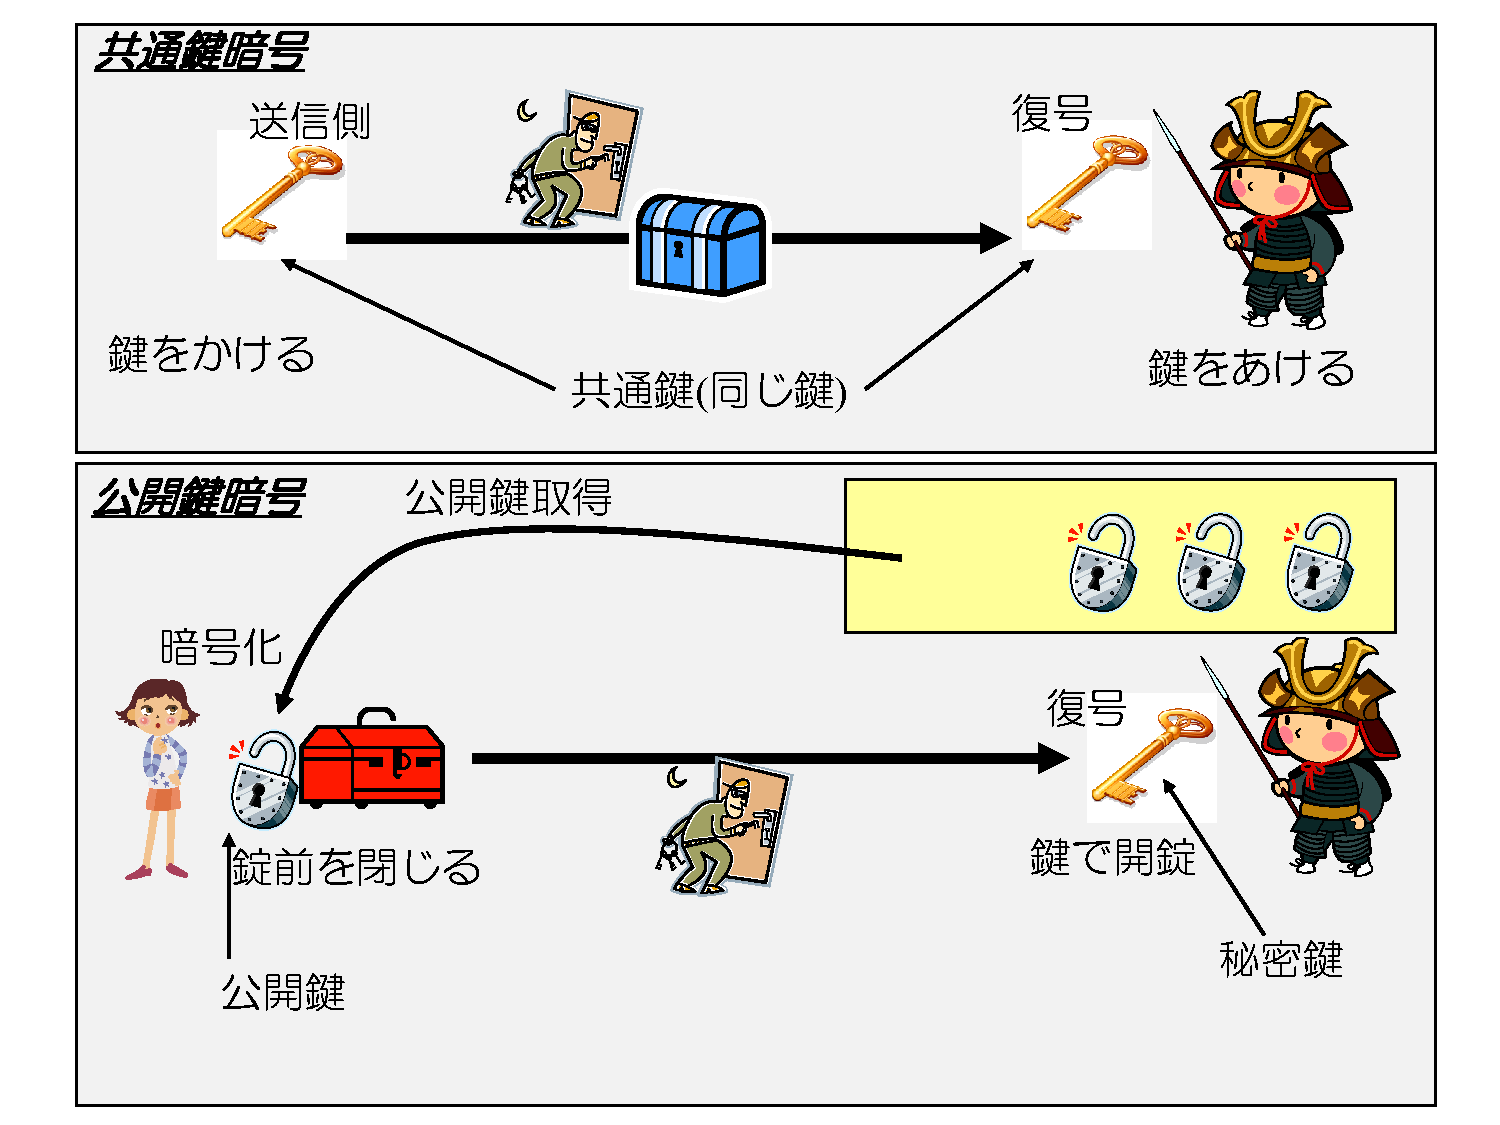
\includegraphics[width=15cm,bb=0 0 720 540,clip]{04_http_auth_crypt/crypt.pdf}
  \label{fig:04:crypt}
  \caption{共通鍵暗号と公開鍵暗号}
 \end{center}
\end{figure}

\subsection{共通鍵暗号}

\begin{description}
 \item[AES] \ \\
            Advanced Encryption Standard の略で,アメリカ政府が策定した標
	    準的な暗号方式である.策定に際して,世界の暗号研究者への公募
	    が行われ,ベルギーの Daemen, Rijmen による Rijndael と呼ばれ
	    た暗号が採用されたので,Rijndael と呼ばれる場合もある.ヨー
	    ロッパ,日本でも標準に採用され,世界的に最も広く使われている
	    暗号方式である.鍵長は,128, 192, 256 ビットから選択できる.
 \item[DES] \ \\
            Data Encryption Standard の略で,AESよりも以前にアメリカで標
	    準だった暗号方式である.設計が古く鍵長が56ビットと短いことも
	    あり,AES に比較すると安全性は低い.また,総当たり以外の解読
	    方法も既に知られている.UNIX OS のパスワードのハッシュ化に用
	    いられたが,現在の UNIX のパスワードのハッシュ化には MD5 を使
	    うことが多い.DES を3回,異なる鍵で暗号化するトリプル
	    DES(3DES, DES3)という派生方式も一時期使われた.
 \item[RC4] \ \\
            Rivest が開発した暗号方式で,無線LANのWEP, WPA, Windows 標準
	    の PPTP 方式 VPN,リモートデスクトッププロトコル,Skype,PDF
	    の暗号化 など,広く用いられている.40ビット(56ビットと呼ばれ
	    ることもある)のものと,104ビット(128ビットと呼ばれることも
	    ある)のものがあるが,40ビットのものは鍵長が短いので現在は使
	    用に適さない.また,128ビットのものでも,総当たり以外の解読方
	    法が知られている.暗号・復号の速度の点から広く使われているが,
	    AES や DES に比較すると安全性は低い.
\end{description}

\subsection{公開鍵暗号}

\begin{description}
 \item[RSA] \ \\
            Rivest, Shamir, Adleman による公開鍵暗号方式の初の実装で,現
	    在でも主流の方式で広く使われている.発明した三者はチューリン
	    グ賞を受賞している.特許により保護されていたので,一時期は他
	    の方式(PGPやDSA)も用いられたが,現在は RSA が一般的である.
 \item[PGP] \ \\
            Zimmermann による公開鍵暗号方式で,フリーソフトウェアとして広
	    く配布され,電子メールの暗号化や,ファイルの暗号化などに用い
	    られることがある.
\end{description}

\section{認証手法}

\subsection{電子署名}

公開鍵暗号は,通信路暗号化に用いる際は,公開鍵で暗号化したものを秘密鍵で
復号するが,逆に秘密鍵で暗号化したものを公開鍵で復号することもできる.

これを利用して,電子署名や認証が実現される.具体的には,ある公開鍵で復号
化できるような暗号を作れる者は,対応する秘密鍵を持つ者のみであるので,公
開鍵に対応する秘密鍵を持つ者が特定できるということから,送信者を特定する
ことができる.第三者が送信者になりすまして,情報を偽造することはできない.

認証や電子署名で用いられる公開鍵のことを,証明書と呼ぶ.

\begin{figure}[ht]
 \begin{center}
  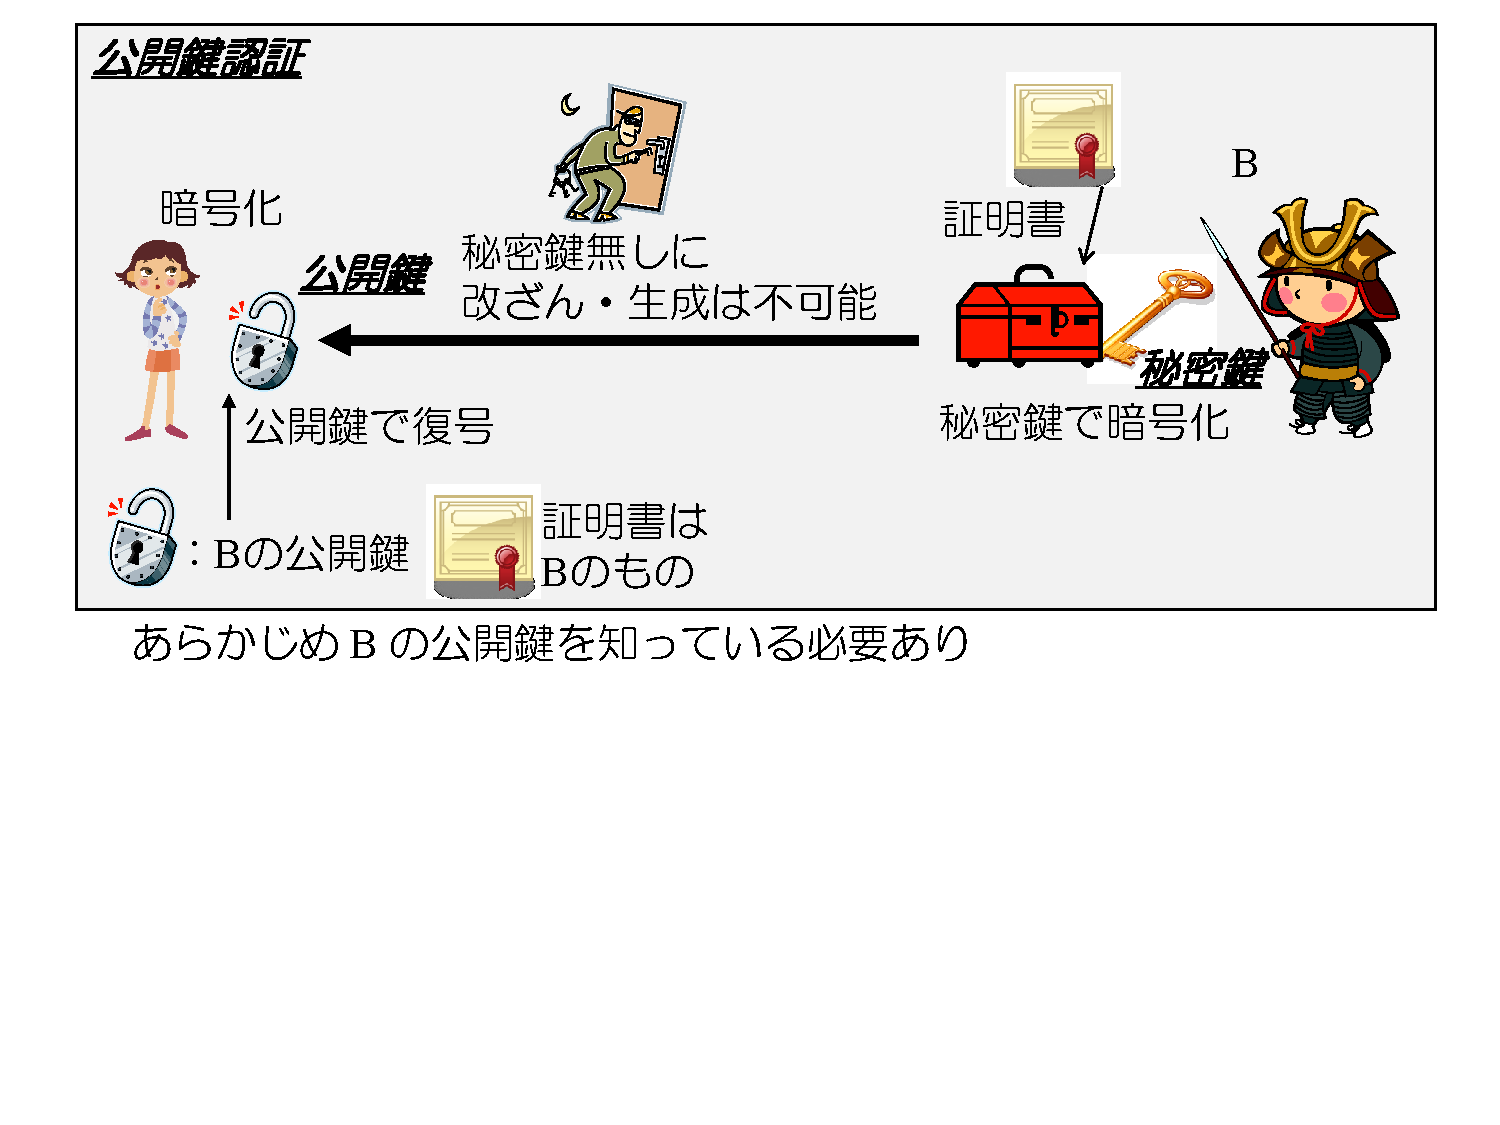
\includegraphics[width=15cm,bb=0 200 720 540,clip]{04_http_auth_crypt/publickey-auth.pdf}
  \label{fig:04:publickey-auth}
  \caption{公開鍵暗号認証}
 \end{center}
\end{figure}

しかし,証明書は確実にある認証対象の送信者であることを保証しなければなら
ない.このためには,ある証明書に対して,対応する秘密鍵を持つ者が誰なのか
を保証するための仕組みが別途必要である.これをPKI (Public Key
Infrastructure) 公開鍵認証基盤と呼ぶ.

一般には,下記のようなものが用いられる.

\begin{enumerate}
 \item 別途,安全な手段で証明書(公開鍵)を取得しておく
 \item 信頼できる第三者により電子署名された公開鍵を取得する
 \item 送信されてきた証明書を,自己申告のまま信頼する
\end{enumerate}

3番目の方法は,実際には個人を認証として用いることはできず,暗号化通信の
みを意図してサーバの公開鍵をそのまま受け入れる,サーバ証明書で使われる程
度である.SSH や HTTPS のサーバ証明書では,簡易運用の際にこの方法もしば
しば用いられる.しかし,問題点としては,悪意を持つ者がサーバのかたったと
しても,その証明書を受け入れてしまうことになり,サーバと認識しながら実は
本来のサーバでない者へ情報を送信することになる.具体的にはログイン・パス
ワード情報を誤って送信してしまうなどがある.これをフィッシング(Phishing)
と呼ぶ.このため,インターネットへ一般公開するサーバなどで用いることは望
ましくない.

そこで,認証を行う際は,証明書の作成者から確実・安全に証明書を送付しても
らう必要がある.SSL では,送信者・受信者ともに確実に信頼できる第三者(そ
の公開鍵=証明書は既知)が,その秘密鍵で証明書を暗号化し,証明書の受信者
は,信頼できる第三者の公開鍵でこの証明書を復号し,復号できた場合は信頼す
る仕組みがある.これを公開鍵基盤と呼ぶ.信頼できる第三者の公開鍵は,あら
かじめ全ての通信者が知っている.信頼できる第三者のことを,認証局
(Certificate Agency: CA)と呼ぶ.具体的には,CAは,ベリサイン社などの公
開鍵の認証を請け負う機関であり,それらの機関の証明書は,Web ブラウザとと
もに配布されている.CAの秘密鍵による,未知の証明書への暗号化を,署名 
(Sign) と呼ぶ.ブラウザとともに配布されすべてのWeb クライアントが既知で
ある証明書のことをルート証明書とよび,ルート証明書を持つ機関を,ルート認
証局あるいは,ルートCAと呼ぶ.

\begin{figure}[ht]
 \begin{center}
  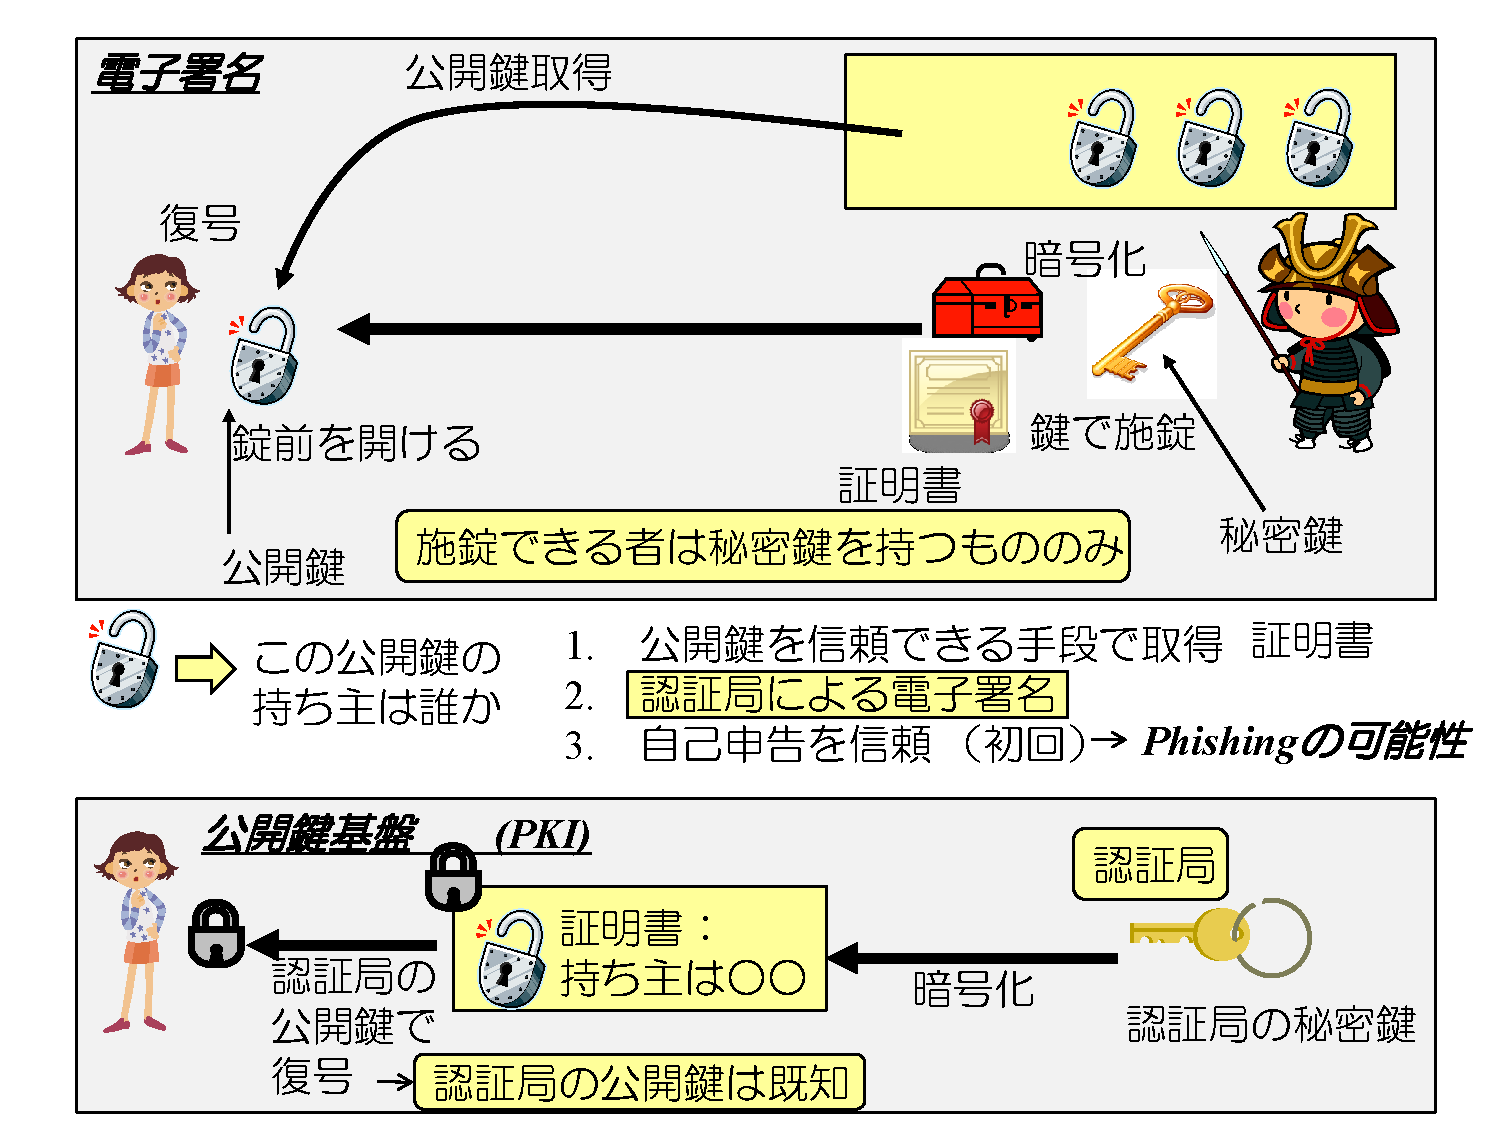
\includegraphics[width=15cm,bb=0 0 720 540,clip]{04_http_auth_crypt/sign.pdf}
  \label{fig:04:sign}
  \caption{認証局による証明書への署名}
 \end{center}
\end{figure}

なお,SSH の公開鍵認証では,認証局による署名の仕組みはなく,安全で信頼性
が確保できる手段であらかじめ公開鍵を送ることを求められる.具体的には,サー
バの管理者宛に,自分の公開鍵を電子メールで送付し,サーバの管理者はその文
面ややりとり,電話などの別の手段での確認などを経て,サーバの所定の保存場
所に,認定された公開鍵として保存される.

\subsection{証明書と認証局}

公開鍵暗号において,ある公開鍵で暗号化したものは特定の秘密鍵を持つ者にし
か復号できないが,公開鍵だけを与えられても受信者が本当の受信者か,本来
の受信者になりすました者かは判定できない.このため,公開鍵で本当に安全な
通信を行うためには,公開鍵を特定の受信者のものであることを証明する仕組み
が必要である.具体的には,ある公開鍵に対して,送信者が信頼できる者が,こ
の鍵が本来の受信者であることを証明する必要がある.

これに用いられるものが,電子署名である.つまり,世界中から信頼される者が,
ある公開鍵に対して,確かに特定の受信者のものであることを証明する.具体的
には,信頼された者(すなわち,公開鍵が分かっている)が,送信者の公開鍵と,
送信者の情報(名前や所属機関など,個人を特定する情報,あるいはホスト名など,
特定のホストであることを特定する情報)の組を,秘密鍵で暗号化する.信頼さ
れた者の公開鍵はわかっているので,これ復号した内容には偽造や改ざんの心
配はない.このため,復号した内容も正しい.これを公開鍵に対する電子署名
(あるいは,単に署名)と呼び,これを保証する内容を証明書と呼ぶ.

「信頼された者」とは,具体的には,認証局サイト(CA)を差し,VeriSign 社を
はじめ,数多くの機関がある.これらの機関の公開鍵と証明書ははじめからブラ
ウザなどにインストールされている.この証明書の信頼関係は,親子関係を作る
ことができるので,信頼された証明書を持つ機関は,別の機関の証明書を発行す
ることができる.

なお,認証局は,各証明書の申請に対して,メールでのやりとりの他,電話や郵
便,クレジットカードの引き落としなどを通して,証明書の保有者の身元を確認
する.

\section{実験内容(1)}

\subsection*{Web サーバの構築}

今回の実験では,世界中で使われており,高機能で安定した動作をする Apache 
を用いて Web サーバを構築する.Server 用のコンピュータに,パッケージシス
テムを用いて Apache (Apache2) をインストールする.

\subsection*{コンテンツの作成と公開}

HTML によるコンテンツを作成し,公開用ディレクトリへ配置する.
その後,Web ブラウザ上でそのコンテンツを表示できることを確認する.

Apache2 の設定ファイルにて \url{http://192.168.0.121/} のように,ファイル名を省略して URI が指定されたときは,index.html ファイルが表示されるようになっており,これを変更することもできる(省略時には別のファイルを表示する,または,ファイル名省略時はエラーを表示する等).ここでは,index.htmlを表示するようにしておく.

\begin{itemize}
 \item Apache2 インストール直後に,\texttt{/var/www/html}の下に\texttt{index.html}としてデフォルトのものがあるので,これが表示できるか確認する
 \item デフォルトの index.html を mv コマンドで別名にリネームする
 \item グループ独自のコンテンツファイルを作成し,index.html として公開する
\end{itemize}


\subsection*{Web サーバでの認証設定}

2種類のアクセス制限(送信元IPアドレス,ユーザ認証)を施したコンテンツを作成する.

\begin{itemize}
 \item コンテンツ公開ディレクトリに,2つのサブディレクトリを作成し,それぞれにコンテンツを作成
 \item 一方のコンテンツディレクトリには HTTP クライアントの接続元の IP アドレスによるアクセス制限
 \item もう一方のコンテンツディレクトリには Basic 認証によるユーザ認証
\end{itemize}

それぞれのアクセス制限の仕様は,下記の通り.
\begin{itemize}
 \item 送信元IPアドレス制限によるものは,グループ内の固定IPアドレスのPC3台のみから閲覧可能にし,それ以外は閲覧できないようにする.
 \item ユーザ認証によるアクセス制限は,HTTP Basic 認証により,限定されたユーザ名とパスワードを入力した場合のみ閲覧できるようにする(グループで決めたユーザ名・パスワードで良い).
\end{itemize}



\textbf{注意! 認証用パスワードは,実験内で平文(ひらぶん)が表示される場
所があるので,普段使用しているものとは異なるものにすること.}

\subsection*{Wireshark によるパケットモニタ}

2種類のアクセス制限の設定を行い,その通信をモニタする.

構築したシステムが正しく意図した動作しているかをパケットモニタで確認する.

Wireshark は高機能パケットキャプチャ(捕捉)・アナライザ(解析)である.
スニファ(嗅ぐ)などとも呼ばれる.LANのパケットを調査する用途に用いるが,
クラッキングツールにも悪用できるものであり,取り扱いには注意する.

プログラムはインターネットからもダウンロードできる.Linux では,apt コマンドなどからもインス
トール可能である.

これを用いて,HTTP のリクエスト・レスポンスの過程や,Basic 認証の際のパ
スワードのパケット内での取り扱いを確認する.

 \begin{itemize}
 \item Wireshark をクライアントにインストールし,サーバへの通信のモニタ
       を行う.
 \item Windows はメインサーバの FTPに,Cent OS はソフトウェアの画面から
       インストールすれば良い.
 \item HTTP 接続にて Basic 認証を行う通信のモニタし,パスワードの情報な
       どを確認する.
 \end{itemize}


\section{実験内容(2)}

\subsection{HTTPS サーバの設定}

HTTP 通信の暗号化を SSL/TLS を用いて行う.

\begin{itemize}
\item SSL/TLS 通信 (HTTPS) 対応設定
\end{itemize}

\subsection{HTTPS 通信のモニタ}

Wireshark によって Windows からサーバへの HTTPS 通信をモニタする.
\begin{itemize}
 \item HTTPS 接続による Basic 認証を行う通信のモニタ
\end{itemize}

HTTP通信がどのようになっているか,Basic 認証の認証情報がどのようになって
いるかを確認する.

\subsection{動的コンテンツ}

動的コンテンツを生成するための設定と動的コンテンツの配置を行う.
\begin{itemize}
\item Apache にて SSI,CGI が実行できる環境の設定
\item 簡単な動的コンテンツの作成
\item PHP の動作環境をサーバに作成
\end{itemize}

簡単な動的なコンテンツの作成として,時刻を表示するプログラムをそ
れぞれ下記の技術を用いて作成し,それぞれの技術的違いを考えてみよ.
\begin{itemize}
 \item SSI
 \item CGI (用いる言語は何でも良いが,本テキストではシェルスクリプトを提供)
 \item PHP
\end{itemize}

次に,CGI でカウンタプログラムを作成せよ.カウンタプログラ
ムはユーザからリクエストを受けるたびに,カウンタの値を1つずつ増加させ,
そのウェブページに何回のリクエストがあったかを表示するものである.プログ
ラムやカウンタを記録するデータファイルの書き込み権限に注意すること.

\section{Apache のインストールと各種設定}

\subsection{Apache のインストール}

Ubuntu への Apache インストール方法について述べる.

スーパーユーザになって下記を実行する.
\begin{cli}
# apt install apache2
\end{cli}

以上で,インストールは終了し起動している.ps コマンドでプロセスを確認する.
\begin{cli}
# ps auxww

 → apache プロセスの行があるかを確認

(行が長くて流れる場合は,パイプ「|」で出力内容を grep コマンドに渡し,
grep コマンドで「apache」の行が残るところのみを抜き出し表示する)

# ps auxww | grep apache

\end{cli}

apache2 プロセスがいくつか動作していることを確認する.もしない場合は,インストールに失敗しているか,実行に失敗している.

\begin{cli}
# ps auxww | grep apache2
root      4873  ...  起動時刻 /usr/sbin/apache2 -k start
www-data  4876  ...  起動時刻 /usr/sbin/apache2 -k start
www-data  4877  ...  起動時刻 /usr/sbin/apache2 -k start
\end{cli}

systemctl コマンドでも下記のように確認できる.

\begin{cli}
# systemctl | grep apache2
apache2.service loaded active running  The Apache web server

# systemctl status apache2

Active: active (running) の行を確認する
\end{cli}

ps コマンドによるプロセス確認が最も信頼できる確認手段であるので,ps コマンドでプロセスが起動していることを,今後も全ての実験内容で確認するのが良い.

起動と終了は,下記で行う.

\begin{cli}
起動
# systemctl start apache2

停止
# systemctl stop apache2

再起動
# systemctl restart apache2
\end{cli}

\subsection{Apache の動作に関連するディレクトリ}

下記に,Ubuntu で配置される主なディレクトリとそこにどのようなファイルが置かれるかを示す.

\begin{description}
 \item[/etc/apache2] \ \\
            設定ファイルがある.apache2.conf が起動時に読み込まれる.
 \item[/etc/apache2/apache2.conf] \ \\ 起動時に読み込まれる設定ファイル.
	    この設定ファイルには全体の構成のみが書かれ,動作する(LISTEN
            する)ポートや,機能の有効化・無効化などは別のファイルを読み
            込むようになっている.全体のデフォルトはここで設定できるので,
	    セキュリティ情報等を他のファイルに引き継ぐよう設定できる.
 \item[/etc/apache2/ports.conf]  \ \\ 動作するポート.デフォルトは TCP
	    80,HTTPS は TCP 443.
 \item[/etc/apache2/sites-available/000-default.conf] \ \\
	    /var/www/html 以下の公開設定などを行う.実際には,
	    apache2.conf の末尾にて sites-enabled のあるファイルが番号順
	    に読み込まれるようになっているが,それらは site-available へ
	    のシンボリックリンクとなっている.
 \item[/var/www/html] \ \\
            公開用ファイル(HTMLファイルや画像ファイル,CGI等のプログ
	    ラムファイル)が置かれる.外部からアクセスされるディレクトリ
	    である.
 \item[/etc/apache2/envvars] \ \\ Apache が動作するユーザ権限や,ログファイルの位置な
	    どを設定する.
 \item[/var/log/apache2] \ \\
            ログファイルがある.アクセスログ・エラーログには常に注意する.
\end{description}

なお,余談であるが,このような配置(デプロイ)は,Debian (Ubuntuの元とな
るディストリビューション)独特のものであり,Debian のパッケージシステム
で,モジュール単位での自動でのコンフィギュレーション,インストール,アン
インストールに対応するためにこのようになっていると,apache2.conf ファイ
ルの冒頭で説明されいる.

Apache をソースコードからコンパイル・インストールすると,デフォルトでは
/usr/local/apache2 以下に全てのプログラム・設定・公開用コンテンツが配置
され,httpd.conf にその設定をすべて記述するようになっている.

\subsection{コンテンツの公開}

/var/www/html 以下に,HTML ファイルを置くことで公開できる.

\subsubsection*{index.html}

index.html は,URI でファイル名が省略されディレクトリ名のみの場合 (URI
が / で終わる場合)に,デフォルトで表示される HTML ファイルである.

通常は,index.html にそのサイトの入り口(ポータル=表玄関)を記述する.

index.html ファイルが無い場合,Apache 設定の Directory /var/www/html の 
Options 設定で,Indexes の項目があれば,そのディレクトリのファイル一覧が
表示される(しばしばこの設定は誤って情報漏洩する原因となるので注意).こ
の項目が無ければ,「403 Forbidden」エラーとなる.

\subsection{HTTP認証(Basic)の設定}

ユーザ・パスワードを入力しての認証つきアクセスの設定は下記のように行う.

まずは,htpasswd でユーザ・パスワードの設定を行う.下記は,ファイル 
.htpasswd にユーザ情報を格納する例である.

\begin{cli}
# htpasswd -c /etc/apache2/.htpasswd testuser
\end{cli}

-c は .htpasswd がまだ無い時に,作成 (create) するオプションで,既に存在
   していれば必要ない."testuser" というユーザを作成し,そのパスワードを
   尋ねてくるので入力する.

/var/www/html の下に basic というディレクトリを作成し,ここにアクセス制
限をかける場合の設定例を示す.

\begin{cli}
# vi /etc/apache2/sites-available/000-default.conf

(下記を <VirtualHost *:80> ディレクティブ内に追加)

<Directory /var/www/html/basic>
        AuthType Basic
        AuthUserFile /etc/apache2/.htpasswd
        AuthName "basic auth"
        
        Satisfy any
        Order deny,allow
        Deny from all
        Require valid-user
</Directory>
\end{cli}

\subsection{IPアドレスによるアクセス制限の設定}

社内専用ページや研究グループ内のみ閲覧可能な内部専用ページの作成には,IPアドレス
よる制限などが用いられる.

/var/www/html の下に inside というディレクトリを作成し,ここにアクセス制
限をかける場合の設定例を示す.

\begin{cli}
# vi /etc/apache2/sites-available/000-default.conf

(下記を <VirtualHost *:80> ディレクティブ内に追加)

<Directory /var/www/html/inside>
        Order deny,allow
        Deny from all
        Allow from サブネット/プレフィックス
</Directory>
\end{cli}

サブネット/プレフィックスには,192.168.100.0/24 のようにアクセスを許可す
る IP アドレスをサブネットおよびサブネットマスクのプレフィックス表記で
設定する.この例では,192.168.100.0から192.168.0.255までのIPアドレスが指定される.

1つしかない場合は,プレフィックスを指定しない.また,2つ以上を指定する場合は,Allow from の行を複数書く.




\subsection{HTTPS による暗号通信設定 (modssl)}

Ubuntu の Apache で SSL/TLS を有効にするために必要なモジュールを使用する
ための設定を行う.

\begin{itemize}
 \item モジュール mod\_ssl を有効にする.
 \item conf ファイルで,SSL を有効化する.
 \item Apache の再起動
\end{itemize}

\begin{cli}
# a2enmod ssl
# a2ensite default-ssl
# systemctl restart apache2
\end{cli}

HTTPS で通信できることを確認する.

ただし,通信そのものは暗号化されているが,証明書は乱数で作成しただけの真
正のものではないため(俗にオレオレ証明書などとも呼ばれる),コミュニティ
内のみの通信であればまだ良いが,このまま公開運用するのは問題がある.

SSL 設定ファイル /etc/apache2/sites-available/default-ssl.conf の下記の2 
行が,それぞれ,証明書(署名された公開鍵),秘密鍵となっていて,現在は,
make-ssl-cert generate-default-snakeoil コマンドが自動的に実行されて作成
された,PEM,KEY ファイルが指定されている.

\begin{cli}
 SSLCertificateFile /etc/ssl/certs/ssl-cert-snakeoil.pem
 SSLCertificateKeyFile /etc/ssl/private/ssl-cert-snakeoil.key
\end{cli}

ブラウザからアクセスした際に,認証されていない証明書である旨の警告が出る
(正規のサイトを詐称しているフィッシングサイトと区別がつかない).

なお,サイトのコンテンツ(DocumentRoot)等の設定内容は,\texttt{000-default.conf}とは別のファイルになるので,内容をあらためて確認し,必要があれば設定を行う\footnote{default-ssl.conf}.


\section{動作確認}

\subsection*{Web サーバ}

全ての設定を終了後,起動を行い,クライアントコンピュータからブラウザを起
動し,ホームページが表示できるか確認する.

また下記を確認する.
\begin{itemize}
 \item URI は設定したドメイン名・ホスト名を使用した URL とする.
 \item 意図したコンテンツが表示されることを確認すること.
 \item アクセス制限(ユーザ認証,IPアクセス制限)をかけたものは,各グルー
       プで別途 URI を指定し,確認を行う.
 ただしくアクセス制限が行えているか,TA などの他のコンピュータなどからの
 アクセスも確認する.
 \item  また,Apache のログも確認し,アクセスの痕跡,アクセスが成功したか否かな
 どを全てチェックし,作業記録に残すこと.意図しないアクセスなどがあればこ
 れも確認する.
 \item HTTPS 通信も確認する.
 \item この時点で,自己署名証明書のため,ブラウザからエラーが出ること,またそのエラーの内容を理解しておく.
  \item Wireshark にて Basic 通信の認証内容(パスワード等)が,HTTP では
       表示され,HTTPS では暗号化されていることを確認する.
\item https でもアクセス制限が同様にかかっているか.
\end{itemize}

\section{考慮すべき点}

\subsection*{WWW・Web サーバ}

\begin{itemize}
 \item HTTP が広く用いられる理由.
 \item データ公開・転送に HTTP を用いる利点・欠点.
 \item バーチャルホストはどのように用いられるか.
 \item 自己署名証明書では,どのようなことは守られ,どのような危険があるか.
\end{itemize}

\clearpage

\subsection*{これまでの確認}

\subsubsection*{サーバの環境変数の設定}

環境変数や良く用いるシェルのコマンドなどを,あらかじめ初期化ファイルに記
述することで,ログイン時に自動的に設定することができる.

初期化ファイルは,Linux 標準シェルの Bash であれば ~/.bashrc,BSD系標準
の Csh であれば ~/.cshrc,商用 UNIX や古い Bsh 系であれば ~/.profile で
ある.

例えば,http\_proxy.https\_proxy を root の環境変数に設定しておきたい場
合は,下記のようにする.

\textbf{(2021年度の情報実験室ではプロキシは必要ない)}

\begin{cli}
$ sudo su  (システムによっては su)
# vi ~/.bashrc

下記を末尾に追記.

export http_proxy=http://proxy.noc.kochi-tech.ac.jp:3128
export https_proxy=http://proxy.noc.kochi-tech.ac.jp:3128
(KUTの場合httpsのプロキシもhttpで指定する)
\end{cli}%$

以上で,毎回入力する必要がなくなる.